\documentclass[12pt]{article}

\usepackage{fullpage}
\usepackage{multicol,multirow}
\usepackage{tabularx}
\usepackage{ulem}
\usepackage[utf8]{inputenc}
\usepackage[russian]{babel}
\usepackage{amsmath}
\usepackage{amssymb}
\usepackage{graphicx}
\graphicspath{./}
\usepackage{color}
\usepackage{titlesec}

\titleformat{\section}
  {\normalfont\Large\bfseries}{\thesection.}{0.3em}{}

\titleformat{\subsection}
  {\normalfont\large\bfseries}{\thesubsection.}{0.3em}{}

\titlespacing{\section}{0pt}{*2}{*2}
\titlespacing{\subsection}{0pt}{*1}{*1}
\titlespacing{\subsubsection}{0pt}{*0}{*0}
\usepackage{listings}
\lstloadlanguages{Lisp}
\lstset{extendedchars=false,
	breaklines=true,
	breakatwhitespace=true,
	keepspaces = true,
	tabsize=2
}
\begin{document}


\section*{Отчет по лабораторной работе №\,2 
по курсу \guillemotleft  Функциональное программирование\guillemotright}
\begin{flushright}
Студент группы 8О-308 МАИ \textit{Балес Александр}, \textnumero 3 по списку \\
\makebox[7cm]{Контакты: {\tt aleks\_bales@mail.ru} \hfill} \\
\makebox[7cm]{Работа выполнена: 01.04.2016 \hfill} \\
\ \\
Преподаватель: Иванов Дмитрий Анатольевич, доц. каф. 806 \\
\makebox[7cm]{Отчет сдан: \hfill} \\
\makebox[7cm]{Итоговая оценка: \hfill} \\
\makebox[7cm]{Подпись преподавателя: \hfill} \\

\end{flushright}

\section{Тема работы}
Простейшие функции работы со списками Коммон Лисп.

\section{Цель работы}
Научиться конструировать списки, находить элемент в списке, использовать схему линейной и древовидной рекурсии для обхода и реконструкции плоских списков и деревьев.

\section{Задание(вариант 2.37)}
Запрограммируйте на языке Коммон Лисп функционал {\color{red}\tt{map-set (f X)}}, аргументами которого являются функция одного аргумента \tt{f} и список \tt{X}, рассматриваемый как множество. Результатом вызова должно быть множество из результатов применения \tt{f} к каждому из элементов \tt{X}. В списки, представляющие множества, нет повторений, а порядок элементов не имеет значения

\section{Оборудование студента}
Процессор Intel Core i5-3210 4\,@\,2.5GHz, память: 8192Mb, разрядность системы: 64.

\section{Программное обеспечение}
ОС Ubuntu 14.04, среда GNU Common Lisp 2.6.10

\section{Идея, метод, алгоритм}
Написал две вспомогательных ф-ии, одна из которых --- {\color{blue}\tt{iterator}}, реализация итерации по списку при помощи рекурсии ("откусывать" голову списка, и рекурсивно вызывать для хвоста); а вторая ф-ия --- {\color{blue}\tt{comp-elem}}, пробегается каждый раз с текущего место в списке и до конца, проверяя на совпадение элементы, причемы перед проверкой применяется ф-ия \tt{f}, которая передается в качестве формального параметра.

\section{Сценарий выполнения работы}
\section{Распечатка программы и её результаты}
\lstinputlisting{./lr2.lsp}
\subsection{Результаты}
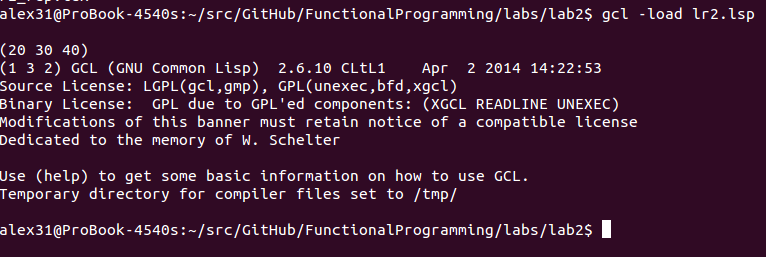
\includegraphics[scale=0.7]{lr2Screen}

%\subsection{Результаты работы}
%\lstinputlisting{./log2.lsp}

\section{Дневник отладки}
\begin{tabular}{|c|p{5cm}|p{5cm}|p{3cm}|}
\hline
Дата & Событие & Действие по исправлению & Примечание \\
\hline
07.04.2016 & Оптимизация & Добавил ф-ию {\color{red}\tt{genList}}, которая возвращает список
из исходных элементов, применяя к ним ф-ию, передаваемую в {\color{red}\tt{map-set}} первым аргументом.
& Асимптотически сложность не изменилась, но по времени должно работать быстрее \\
\hline 
\end{tabular}

\section{Замечания, выводы}
Из распечатки программы сразу видно, что сложность программы по времени $O(N^2)$, где $N$ --- число элементов в списке. Стоит сразу также отметить, что ф-ии {\color{blue}\tt{iterator, comp-elem}} реализованы при помощи концевой рекурсии, а это значит, что скорее всего, компилятор Коммон Лисп их оптимизирует до простого цикла. По памяти так же сложность составляет $O(N^2)$, т.к. мы при каждом рекурсивном вызове передаем в качестве параметром списки длины $N +$ генерируется новый список из неповторяющихся элементов.
\end{document}
